\section*{6.4 Efficient Parallelization of AlphaBeta}

\subsection*{1.}
In the lecture, most of those questions were already answered. A minimal tree looks like that: Every node (=move) has several children. It always has to evaluate the leftmost child in order to get initial values. Also, their values are assumed to be the best, as they represent the best moves. This is due to the iterative deepening. A leftmost child is therefore called ``all node'', because the depthsearch has to descent in every single child of them. Other nodes are then called ``cut nodes'', as their children (except the leftmost) most likely do not have to be evaluated and therefore can be cut off. The process still has to descent into them, as they are children of ``all nodes'', but all of their children (minus the leftmost of them, which again is an ``all node'', can, and if the assumptions that the moves are perfectly ordered hold, will be pruned. Slides 5 to 7 of the presentation of the lecture show how such a tree looks like in picture.
A decomposition strategy presented in the lecture (and used in this task) is pvsplit, which uses somewhat a bottom up approach: First, the tree is traversed down along the principal variation, until the depthsearch reaches the maximum depth. The principal variation is the sequence of best moves, which has been determined with iterative deepening (We first evaluate the position with maxdepth1, order moves by the results, then go with maxdepth2, again order the moves, etc.). At this point, all children of this node are evaluated by the worker processes, and their values is returned to the master. After that, the main process traverses up one step, and again distributes the work on the children of that node to the workers. However, it already knows the value of the leftmost child, as this was already evaluated in the previous step, and therefore searchoverhead should be reduced. This is repeated until the algorithm reaches the topmost layer of the tree and has evaluated the children of the root node (which obviously is also an all node, as the current boardposition is included in the best movesequence). By doing this, we can assure that we never will start depthsearch with a broad window and high depth on too many processes, and therefore should reduce search overhead significantly. In fact, the adaptive search window also helps tremendously at achieving this. This decomposition strategy only works for alphabeta implementations with iterative deepening, as otherwise it is very difficult to determine the principal variation.

Note that the number of processes influences the amount of search overhead. The more processes, the more depthsearches get startet concurrently with an old alphabeta window, which leads to unnecessary evaluations.

\begin{center}
  \begin{tabular}{|r|r|r|}
    \hline
    Setting & AlphaBeta & Overhead pvsplit (4p)\\ \hline
    startposition, depth5 & 589,038 & 5.8\% (623,022 evals)  \\ \hline
    midgame1, depth5 & 4,120,198 & 7.0\% (4,410,253 evals)  \\ \hline
    midgame2, depth5 & 2,067,878 & 13.2\% (2,340,727 evals)   \\ \hline
    endgame, depth5 & 402,920 & 8.3\% (436,358 evals)   \\ \hline
  \end{tabular}
\end{center}


\subsection*{2. Speedup figures}
In this setting, we are using the runtime of the evaluation of the sequential version distributed to the students as a baseline, and then compare this to the runtime of our parallelization. Note that you should not use evalrate to determine speedup, because you might have (more precisely: do have) search overhead, and this would make your parallelization look a lot better than it actually is.
You can see that the parallelization does a pretty decent job, although the speedup by no means is perfect.  There is also a pretty obvious correlation between problem complexity and maximum achievable speedup: midgame1, which is by far the most complex position, peaks around speedup 3, while endgame, which is the most simple position, has a speedup of close to 7 on 8 workers.

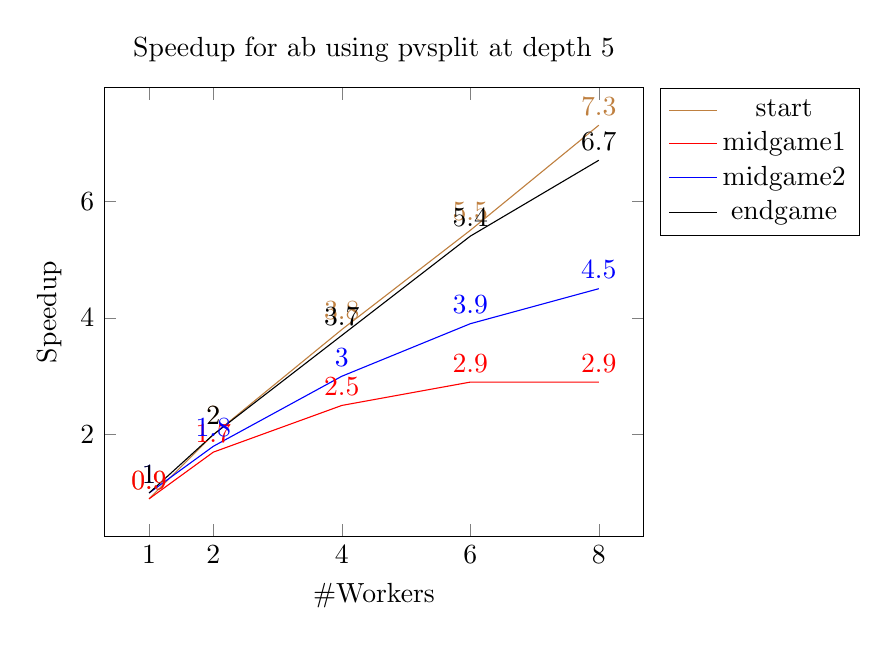
\begin{tikzpicture}
  \begin{axis}[
      legend style={cells={align=left}},
      xtick={1, 2, 4, 6, 8},
      xlabel=\#Workers,
      ylabel=Speedup,
      title=Speedup for ab using pvsplit at depth 5,
      legend pos = outer north east,
      nodes near coords,
      scaled ticks = false,
      y tick label style={
        /pgf/number format/.cd,
	fixed,
        fixed zerofill,
	precision=0,
        /tikz/.cd
      },
      no markers]
     \addplot[color=brown] coordinates {
       (1,0.9)
       (2,2.0)
       (4,3.8)
       (6,5.5)
       (8,7.3)
     };
    \addplot[color=red] coordinates {
       (1,0.9)
       (2,1.7)
       (4,2.5)
       (6,2.9)
       (8,2.9)
     };
     \addplot[color=blue] coordinates {
       (1,1.0)
       (2,1.8)
       (4,3.0)
       (6,3.9)
       (8,4.5)
     };
     \addplot[color=black] coordinates {
       (1,1.0)
       (2,2.0)
       (4,3.7)
       (6,5.4)
       (8,6.7)
     };
     \legend{start, midgame1, midgame2, endgame}
  \end{axis}
  
\end{tikzpicture}
